\documentclass[10pt,a4paper]{article}
\usepackage[T1]{fontenc}
\usepackage{lmodern}
\usepackage[margin=2.1cm]{geometry}
\usepackage{amsmath,amssymb}
\usepackage{graphicx}
\usepackage{booktabs}
\usepackage{xcolor}
\usepackage[font=small,labelfont=bf]{caption}
\usepackage[colorlinks=true,linkcolor=black,urlcolor=blue,citecolor=black]{hyperref}
\usepackage{enumitem}
\usepackage{microtype}
\graphicspath{{figures/}}
\setlist{nosep,leftmargin=1.4em}
\newcommand{\C}{\,^\circ\mathrm{C}}
\newcommand{\TEAMNAME}{\textbf{Team Bueno}\\ Evan Tobias \quad$\cdot$\quad Krishna Gaur \quad$\cdot$\quad James Joshua}
% Every number quoted below is written by scripts/run_analysis.py into numbers.tex and the table_*.tex files.
% Generated by scripts/run_analysis.py -- do not edit by hand.
\newcommand{\BattMinusTankAC}{0.9}
\newcommand{\BattMinusTankWC}{$-$14.9}
\newcommand{\CleanerAC}{16}
\newcommand{\CleanerWC}{0}
\newcommand{\CopNightAC}{3.19}
\newcommand{\CopNightWC}{5.69}
\newcommand{\CopRefAC}{2.93}
\newcommand{\CopRefWC}{6.48}
\newcommand{\CopSolarAC}{2.76}
\newcommand{\CopSolarWC}{5.85}
\newcommand{\DTdb}{5.0}
\newcommand{\DTdbDubai}{3.6}
\newcommand{\DTdbNormals}{7.3}
\newcommand{\DTdbReanA}{7.2}
\newcommand{\DTdbReanB}{7.8}
\newcommand{\DTdbSharjah}{5.5}
\newcommand{\DTdp}{$-$4.6}
\newcommand{\DTdpAbs}{4.6}
\newcommand{\DTdpDubai}{$-$1.6}
\newcommand{\DTdpNormals}{0.0}
\newcommand{\DTdpReanA}{$-$6.0}
\newcommand{\DTdpReanB}{$-$6.5}
\newcommand{\DTdpSharjah}{$-$2.1}
\newcommand{\DTwb}{$-$1.4}
\newcommand{\DTwbAbs}{1.4}
\newcommand{\DTwbFromDb}{1.3}
\newcommand{\DTwbFromDp}{$-$2.9}
\newcommand{\DTwbTwoTerm}{$-$1.6}
\newcommand{\DampA}{0.26}
\newcommand{\DampB}{0.62}
\newcommand{\DaysAC}{39}
\newcommand{\DaysWC}{100}
\newcommand{\DesignUnderAC}{27}
\newcommand{\EffAC}{84.1}
\newcommand{\EffRoundAC}{84}
\newcommand{\EffRoundWC}{100}
\newcommand{\EffWC}{99.9}
\newcommand{\ErrClassAC}{2.2}
\newcommand{\ErrClassHiAC}{2.8}
\newcommand{\ErrClassHiWC}{6.3}
\newcommand{\ErrClassWC}{2.6}
\newcommand{\ErrOwnAC}{1.7}
\newcommand{\ErrOwnWC}{1.3}
\newcommand{\ErrTestAC}{1.9}
\newcommand{\ErrTestWC}{2.3}
\newcommand{\FirstDTdb}{7.3}
\newcommand{\FirstDTwb}{1.7}
\newcommand{\FirstPiAC}{18.5}
\newcommand{\FirstPiACLibraryChiller}{24.6}
\newcommand{\FirstPiACMeasuredWeather}{11.9}
\newcommand{\FirstPiWC}{3.5}
\newcommand{\IceAC}{61}
\newcommand{\IceLossAC}{23}
\newcommand{\IceLossWC}{23}
\newcommand{\IceWC}{76}
\newcommand{\IdealOverWC}{66}
\newcommand{\IdealUnderAC}{19}
\newcommand{\LiftAC}{35.3}
\newcommand{\LiftHiAC}{36.4}
\newcommand{\LiftHiWC}{47.6}
\newcommand{\LiftLoAC}{35.1}
\newcommand{\LiftLoWC}{41.0}
\newcommand{\LiftNightAC}{32.5}
\newcommand{\LiftNightWC}{49.6}
\newcommand{\LiftPhysAC}{44}
\newcommand{\LiftPhysWC}{26}
\newcommand{\LiftTrainAC}{36.1}
\newcommand{\LiftTrainWC}{44.2}
\newcommand{\LiftWC}{43.6}
\newcommand{\MaxGap}{4}
\newcommand{\MaxMissing}{50}
\newcommand{\McHiAC}{86}
\newcommand{\McHiWC}{102}
\newcommand{\McLoAC}{78}
\newcommand{\McLoWC}{93}
\newcommand{\McMedAC}{82}
\newcommand{\McMedWC}{97}
\newcommand{\McWinsAC}{25}
\newcommand{\McWinsWC}{100}
\newcommand{\NAC}{111}
\newcommand{\NDays}{1460}
\newcommand{\NMachines}{268}
\newcommand{\NSeasonDays}{736}
\newcommand{\NStationYears}{4}
\newcommand{\NTestAC}{56}
\newcommand{\NTestWC}{79}
\newcommand{\NTotalAC}{111}
\newcommand{\NTotalWC}{162}
\newcommand{\NTrainAC}{55}
\newcommand{\NTrainWC}{78}
\newcommand{\NWC}{157}
\newcommand{\NormRangeNormals}{14.0}
\newcommand{\NormRangeObs}{10.9}
\newcommand{\NormTmaxAbsMax}{1.7}
\newcommand{\NormTmaxDiff}{0.5}
\newcommand{\NormTminDiff}{3.2}
\newcommand{\NormTminDiffHi}{4.5}
\newcommand{\NormTminDiffLo}{1.9}
\newcommand{\PiAC}{15.5}
\newcommand{\PiACDubai}{10.8}
\newcommand{\PiACNormals}{24.6}
\newcommand{\PiACReanA}{23.8}
\newcommand{\PiACReanB}{25.2}
\newcommand{\PiACSharjah}{17.3}
\newcommand{\PiAbsAC}{15.5}
\newcommand{\PiAbsWC}{2.8}
\newcommand{\PiMaxAC}{16.9}
\newcommand{\PiMaxWC}{$-$2.3}
\newcommand{\PiMinAC}{14.4}
\newcommand{\PiMinWC}{$-$3.0}
\newcommand{\PiMonthMaxAC}{22.0}
\newcommand{\PiMonthMaxWC}{1.4}
\newcommand{\PiMonthMinAC}{12.3}
\newcommand{\PiMonthMinWC}{$-$4.0}
\newcommand{\PiStar}{14.1}
\newcommand{\PiWC}{$-$2.8}
\newcommand{\PiWCDubai}{$-$0.0}
\newcommand{\PiWCNormals}{3.5}
\newcommand{\PiWCReanA}{$-$3.0}
\newcommand{\PiWCReanB}{$-$3.5}
\newcommand{\PiWCSharjah}{0.7}
\newcommand{\PiYearAC}{16.7}
\newcommand{\PiYearWC}{$-$1.4}
\newcommand{\RStarAC}{0.84}
\newcommand{\RStarWC}{1.00}
\newcommand{\RangeAC}{9.8}
\newcommand{\RangeDb}{9.8}
\newcommand{\RangeWC}{5.0}
\newcommand{\RangeWb}{5.0}
\newcommand{\RealOverIdealAC}{24}
\newcommand{\RealOverIdealWC}{40}
\newcommand{\RouteBattAC}{369}
\newcommand{\RouteBattWC}{207}
\newcommand{\RouteGridAC}{314}
\newcommand{\RouteGridWC}{176}
\newcommand{\RouteTankAC}{373}
\newcommand{\RouteTankWC}{176}
\newcommand{\SavingAC}{1}
\newcommand{\SavingWC}{15}
\newcommand{\SecondLawHiAC}{61}
\newcommand{\SecondLawHiWC}{69}
\newcommand{\SecondLawLoAC}{44}
\newcommand{\SecondLawLoWC}{48}
\newcommand{\SensAC}{2.83}
\newcommand{\SensHiAC}{2.89}
\newcommand{\SensHiWC}{2.99}
\newcommand{\SensIdealAC}{2.3}
\newcommand{\SensIdealWC}{3.8}
\newcommand{\SensLoAC}{2.67}
\newcommand{\SensLoWC}{1.73}
\newcommand{\SensWC}{2.30}
\newcommand{\SwingAC}{5.0}
\newcommand{\SwingStarAC}{4.6}
\newcommand{\SwingStarWC}{7.0}
\newcommand{\SwingWC}{$-$1.4}
\newcommand{\TMean}{34.2}
\newcommand{\TRefAC}{35.0}
\newcommand{\TRefWC}{19.9}
\newcommand{\TdMean}{21.6}


\title{\vspace{-1.2cm}\textbf{The Carnot Penalty}\\[2pt]
\large When should the Gulf make its cold? A thermodynamic model of solar-following cold storage in Abu Dhabi}
\author{\TEAMNAME \\ \small Carnot 2026 \quad$\cdot$\quad Afkar 2026, IIT Delhi -- Abu Dhabi \quad$\cdot$\quad 14 November 2026\\
\small Revised version. Section~\ref{sec:changed} lists what changed since the submission of 13 November.}
\date{}

\begin{document}
\maketitle
\vspace{-0.9cm}
\begin{abstract}\noindent
The UAE grid is filling up with midday solar power, while most of its summer electricity goes to cooling
that is still needed long after sunset. An obvious idea is to run chillers at solar noon and store the cold
in a water tank. But noon is also when the outdoor air is hottest, so a chiller should then be at its
\emph{least} efficient. We call the extra electricity this costs the \textbf{Carnot penalty}~$\pi$ and show that,
for a chiller whose work per unit of cold is linear in the heat-sink temperature, it has an exact closed form:
$\pi=\Delta T_{\text{sink}}/L_{\text{night}}$, the solar-minus-night difference in sink temperature divided by
the night-time temperature lift. Two one-line decision rules follow: a cold tank beats a battery on energy if
$\pi<\eta_{\text{tank}}/\eta_{\text{batt}}-1$ (14\%), and solar-following cold storage cuts emissions if solar-hour
electricity is cleaner than night electricity by a factor $r^*=\eta_{\text{tank}}/(1+\pi)$.
We calibrate the chiller model on \NMachines{} real machines (\NWC{} water-cooled, \NAC{} air-cooled) and evaluate it
on \NDays{} measured days: four station-years of hourly airport observations in Abu Dhabi.
\textbf{Result:} an air-cooled chiller pays $\pi\approx$ \PiAC\%, so a cold tank returns \EffRoundAC\% of the solar
electricity put into it, level with a lithium-ion battery (85\%). A water-cooled (district-cooling) plant pays
nothing: $\pi\approx$ \PiWC\%, a small bonus, so its tank returns about \EffRoundWC\% and beats the battery on every
day of the cooling season. The reason is in the humidity. A cooling tower rejects heat to the wet-bulb
temperature, which follows the dry-bulb only weakly (\DampA~K per K) and the dew point strongly (\DampB~K per K),
and in Abu Dhabi the dew point falls by \DTdpAbs~K in the solar hours. The first version of this model, built on a
synthetic year from monthly normals, missed that effect; testing it against measurements is what found it.
\end{abstract}

\section{The problem and why it matters}
On very hot days space cooling can exceed 70\% of peak residential electricity demand in parts of the Middle
East~\cite{iea}. At the same time Abu Dhabi's supply is changing shape: the Barakah nuclear plant (four 1.4~GW units)
runs flat around the clock, gigawatt-scale solar parks such as Al Dhafra (2~GW) produce only in daytime, and in 2025
Abu Dhabi announced a 5.2~GW solar plant coupled to 19~GWh of batteries to deliver 1~GW around the clock~\cite{rtc}.
Clean electricity is therefore most abundant around noon, but a large part of the cooling demand falls in the
evening and night, when the buildings are still hot and the sun is gone.

Solar energy can be moved to the night in two ways: store \emph{electricity} in a battery and run the chiller at
night, or run the chiller at noon and store \emph{cold} in an insulated chilled-water tank (district-cooling plants in
the UAE already use such tanks for peak shaving). The second route looks cheaper and simpler, but it forces the
chiller to work when the outdoor air is hottest. \textbf{Our question:} how large is that thermodynamic handicap in
Abu Dhabi, what does it depend on, and when is storing cold still the better choice?

\paragraph{Related work and what is new.} Storing solar electricity as cold instead of in batteries has been compared
before: for stand-alone photovoltaic chillers~\cite{wang2020}, for photovoltaic air-conditioning with phase-change
storage in different climates~\cite{wangdennis}, for off-grid cooling in the tropics on life-cycle
cost~\cite{luerssen}, and for the power system of Qatar with ice storage~\cite{alaali}. These are numerical studies
of particular systems. Our contribution is different in kind:
(i) we define the Carnot penalty and prove an exact closed form for it (Eq.~\ref{eq:pi});
(ii) we derive two one-line decision rules, cold tank versus battery (Eq.~\ref{eq:batt}) and solar-following versus
night production (Eq.~\ref{eq:clean});
(iii) we show with measured weather that the heat sink of a cooling tower in Abu Dhabi is \emph{cooler} in the solar
hours than at night, explain it with a two-term response of the wet-bulb temperature (Eq.~\ref{eq:twb}), and so find
that district-cooling plants pay no thermodynamic price for following the sun;
(iv) we calibrate both chiller classes on \NMachines{} real machines and show that the textbook ``constant fraction
of Carnot'' model misjudges their temperature sensitivity in opposite directions.
We are not aware of a previous statement of (i)--(iii) in this form. This is new work prepared for this competition;
nothing here has been published before.

\section{Model}
\subsection{Chiller}
A chiller moves heat from an evaporator at temperature $T_e$ to a condenser at $T_c$. The Carnot limit is
$\mathrm{COP}_{\text{Carnot}}=T_e/(T_c-T_e)$ (kelvin), and a real machine achieves a fraction of it. The condenser
must sit above the outdoor heat sink, $T_c=T_s+a$, where $T_s$ is the \emph{dry-bulb} temperature for an air-cooled
chiller and the \emph{wet-bulb} temperature for a water-cooled chiller with a cooling tower, and $a$ is a fixed
approach. With $T_e$ fixed by the chilled-water temperature, the electricity needed per unit of cold is linear in the
sink temperature:
\begin{equation}
w(T_s)\equiv\frac{1}{\mathrm{COP}(T_s)}=\frac{L_0+(T_s-T_0)}{\mathrm{COP}_0\,L_0},
\label{eq:w}
\end{equation}
where $\mathrm{COP}_0$ is the COP at a reference sink temperature $T_0$ and $L_0$ is the \emph{effective lift} at that
point. The model has one shape parameter, $L_0$, with a direct meaning: the COP falls by $s=1/L_0$ per kelvin of
sink temperature. $L_0$ is fitted to real machines (Sec.~\ref{sec:cal}); it is not a physical temperature difference.

\subsection{Heat sinks: dry-bulb and wet-bulb}
The wet-bulb temperature $T_{wb}$ is obtained from dry-bulb $T$ and humidity ratio $W$ by solving the
adiabatic-saturation energy balance~\cite{ashrae},
$W=\dfrac{(2501-2.326\,T_{wb})\,W_s(T_{wb})-1.006\,(T-T_{wb})}{2501+1.86\,T-4.186\,T_{wb}}$,
by bisection, with saturation pressure from the Magnus form~\cite{magnus}. The moisture content is set by the dew
point $T_d$ through $W=W_s(T_d)$. Differentiating the balance gives the response of the wet-bulb temperature to
changes in the dry-bulb and in the dew point:
\begin{equation}
\Delta T_{wb}\approx a\,\Delta T+b\,\Delta T_d,\qquad
a=\Big[1+\frac{h_{fg}}{c_p}\,W_s'(T_{wb})\Big]^{-1},\qquad
b=(1-a)\,\frac{W_s'(T_d)}{W_s'(T_{wb})},
\label{eq:twb}
\end{equation}
with $h_{fg}$ the latent heat of water, $c_p$ the specific heat of moist air and $W_s'$ the slope of the saturation
humidity ratio. At the mean cooling-season state of Abu Dhabi (\TMean$\C$, dew point \TdMean$\C$) this gives
$a=$ \textbf{\DampA} and $b=$ \textbf{\DampB}: a cooling tower sees only a quarter of any dry-bulb swing, but more
than half of any dew-point swing.

\subsection{The Carnot penalty}
Let cold be \emph{made} with hourly weights $m_t$ (we use the solar irradiance, so production follows the sun) and
\emph{used} with weights $u_t$ (the dark hours). Because $w$ in Eq.~\eqref{eq:w} is linear, the weighted mean of $w$
equals $w$ evaluated at the weighted mean sink temperature, $\bar T_m$ or $\bar T_u$. The Carnot penalty, defined as
the relative extra electricity for making cold at solar hours instead of on demand at night, is therefore
\begin{equation}
\boxed{\;\pi\equiv\frac{\sum m_t w_t/\sum m_t}{\sum u_t w_t/\sum u_t}-1
=\frac{\bar T_m-\bar T_u}{L_0+\bar T_u-T_0}=\frac{\Delta T_{\text{sink}}}{L_{\text{night}}}\;}
\label{eq:pi}
\end{equation}
This is an identity, not an approximation: the code confirms it to better than $10^{-12}$ on all \NDays{} measured
days (Fig.~\ref{fig:cf}a). Nothing forces $\pi$ to be positive: if the sink is cooler in the solar hours than at
night, following the sun \emph{saves} electricity. If charging also needs colder water (evaporator lowered by
$\delta$, e.g.\ $\delta\approx12$~K for ice), the numerator gains $\delta$.

\subsection{Cold tank or battery?}
To deliver one unit of night cooling, three routes need the following electricity ($\eta_t$: tank round-trip
efficiency, $\eta_b$: battery round-trip efficiency, $\bar w_u$: night work per unit cold):
grid at night $\bar w_u$;\; solar $\to$ battery $\to$ chiller at night $\bar w_u/\eta_b$;\; solar $\to$ chiller $\to$
cold tank $\bar w_u(1+\pi)/\eta_t$. Hence the tank is an electricity store with effective round-trip efficiency
$\eta_{\text{eff}}=\eta_t/(1+\pi)$, and
\begin{equation}
\text{cold tank beats battery}\iff\pi<\pi^*=\frac{\eta_t}{\eta_b}-1
\iff\Delta T_{\text{sink}}<\Delta T^*=\pi^*L_{\text{night}} .
\label{eq:batt}
\end{equation}
With $\eta_t=0.97$ and $\eta_b=0.85$~\cite{atb}, $\pi^*=$ \PiStar\%.
If night electricity carries emissions (or price) $e_n$ and solar-hour electricity $e_s$, shifting production to the
sun reduces emissions when
\begin{equation}
r\equiv\frac{e_s}{e_n}<r^*=\frac{\eta_t}{1+\pi},\qquad\text{saving}=1-\frac{r}{r^*}.
\label{eq:clean}
\end{equation}

\subsection{Assumptions}
\begin{center}\small
\begin{tabular}{@{}p{0.3cm}p{6.1cm}p{9.6cm}@{}}
\toprule
 & Assumption & Justification / how it is tested\\
\midrule
A1 & $1/\mathrm{COP}$ is linear in sink temperature with one effective lift $L_0$ per technology & Fitted to \NWC{} water-cooled and \NAC{} air-cooled machines (Sec.~\ref{sec:cal}); median curve errors \ErrClassWC\% and \ErrClassAC\%, out-of-sample \ErrTestWC\% and \ErrTestAC\%\\
A2 & Chillers run at full load & Storage exists precisely so that chillers can run flat out; part-load curves ignored\\
A3 & Fixed approaches (cooling tower 4~K) & A constant offset cancels in $\Delta T_{\text{sink}}$\\
A4 & Stratified chilled-water tank, same supply temperature; $\eta_t=0.97$ & Tested: $\eta_t$ 0.90--0.99, charging water 2~K colder, ice ($\delta=12$~K)\\
A5 & Battery round-trip efficiency $\eta_b=0.85$~\cite{atb} & Monte Carlo range 0.80--0.90\\
A6 & Weather is the measured record of two Abu Dhabi airports, 2022 and 2023 & Tested: each station and each year separately; Dubai and Sharjah as a regional check (Table~\ref{tab:sets})\\
A7 & Night cooling load uniform over the dark hours & Tested: load weighted by degree-hours above 18$\C$\\
A8 & Production follows the irradiance of a reanalysis~\cite{openmeteo} & Tested: clear-sky model~\cite{haurwitz}; flat 09--15~h charging window\\
\bottomrule
\end{tabular}
\end{center}

\section{Data and calibration}\label{sec:cal}
\paragraph{Chillers.} EnergyPlus ships libraries of electric chillers whose performance curves were fitted to
manufacturers' data~\cite{eplus,hydeman}. For water-cooled machines we read all \NTotalWC{}
\texttt{Chiller:Electric:EIR} objects of \texttt{Chillers.idf}, keep the \NWC{} with physically sensible curves, and
for each compute the measured sensitivity $s=-\mathrm{d}\ln\mathrm{COP}/\mathrm{d}T$ at its reference point. The
median is \textbf{\SensWC\,\%/K} (interquartile range \SensLoWC--\SensHiWC), i.e.\ $L_0=$ \LiftWC~K (95\% bootstrap
interval \LiftLoWC--\LiftHiWC~K). For air-cooled machines the same reader takes the \NAC{} chillers of
\texttt{AirCooledChiller.idf}: the median is \textbf{\SensAC\,\%/K} (\SensLoAC--\SensHiAC), i.e.\ $L_0=$ \LiftAC~K
(\LiftLoAC--\LiftHiAC~K), with a reference COP of \CopRefAC{} at \TRefAC$\C$ outdoor air.

A textbook constant-efficiency Carnot fraction using the \emph{physical} lift of the water-cooled machines
(\LiftPhysWC~K) would predict \SensIdealWC\,\%/K, about \IdealOverWC\% too sensitive: real chillers have fixed
internal losses, so their second-law efficiency improves as the lift grows~\cite{gordon}. For the air-cooled machines
the same textbook estimate (condensing 14~K above the outdoor air, lift \LiftPhysAC~K) gives \SensIdealAC\,\%/K, about
\IdealUnderAC\% too \emph{insensitive} (Fig.~\ref{fig:cal}). We therefore keep the linear form of Eq.~\eqref{eq:w} but
use the measured effective lifts. Evaluated with physical temperatures (condensing 7~K above the
entering water or 14~K above the outdoor air, evaporating 1.5~K below the chilled water), the fitted machines run at
\SecondLawLoWC--\SecondLawHiWC\% (water-cooled) and \SecondLawLoAC--\SecondLawHiAC\% (air-cooled) of the Carnot COP over
every measured hour, so the second law is respected.
With a single $L_0$ per class the model reproduces each machine's COP curve from 8~K below to 10~K above its
reference with a median RMS error of \ErrClassWC\% (water-cooled; 90th percentile \ErrClassHiWC\%) and \ErrClassAC\%
(air-cooled; \ErrClassHiAC\%); with each machine's own $L_0$ the errors are \ErrOwnWC\% and \ErrOwnAC\%, which tests
the functional form itself. Calibrating on a random half and testing on the other half gives $L_0=$ \LiftTrainWC~K
with a median error of \ErrTestWC\% (\NTrainWC{} machines to fit, \NTestWC{} to test) and $L_0=$ \LiftTrainAC~K with
\ErrTestAC\% (\NTrainAC{} and \NTestAC).

\begin{figure}[h]\centering
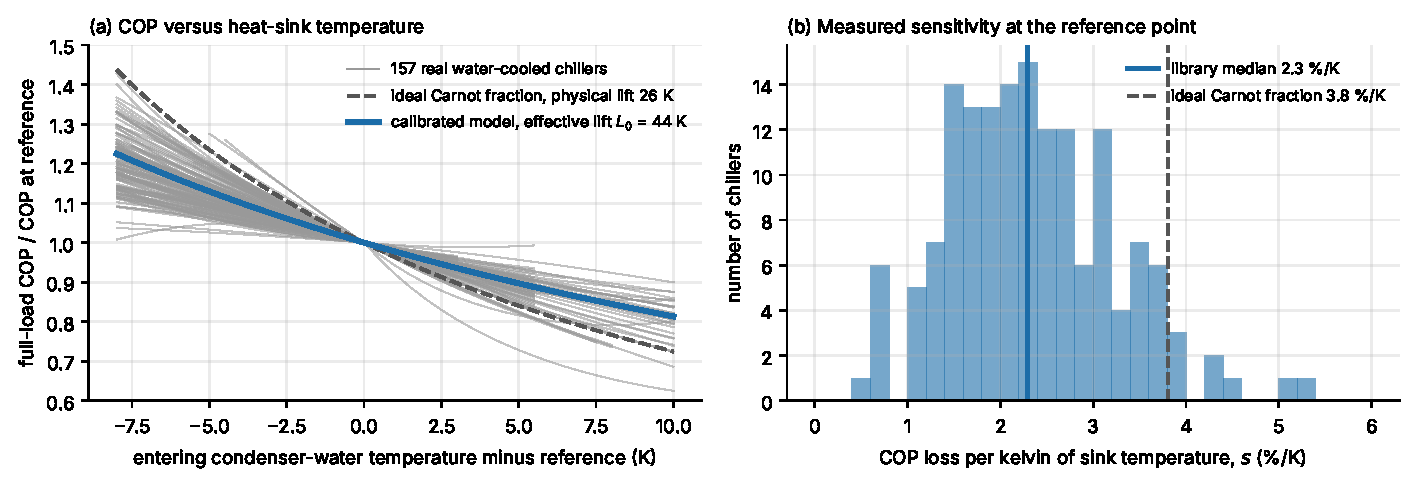
\includegraphics[width=\linewidth]{fig2_chiller_calibration.pdf}
\caption{Calibration on real machines. (a, b) COP of the library chillers against heat-sink temperature (grey), the
ideal Carnot-fraction prediction (dashed) and the calibrated model. (c) Distribution of measured sensitivity.}
\label{fig:cal}
\end{figure}

\paragraph{Weather.} Hourly dry-bulb and dew-point temperatures come from the routine airport weather reports
archived by the Iowa Environmental Mesonet~\cite{iem}: Abu Dhabi International Airport, on the mainland, and
Al Bateen airport, on Abu Dhabi island, for 2022 and 2023. That is \NDays{} days, \NSeasonDays{} of them in the
cooling season (May--October). In no station-year are more than \MaxMissing{} of the 8760 hours missing (longest gap
\MaxGap~h); they are interpolated. Airports do not report irradiance, which the model needs only as hourly weights,
so the weights come from a reanalysis~\cite{openmeteo}; a clear-sky model gives the same answer
(Sec.~\ref{sec:unc}). Dubai and Sharjah airports (2023) serve as a regional check.
Fig.~\ref{fig:sinks} shows what the record says. Over May--October the dry-bulb is \DTdb~K warmer in the solar hours
than at night. The dew point is \DTdpAbs~K \emph{lower}: the surface air dries out in the heat of the day and the
humid Gulf air returns in the evening (we report this observation; we do not model its cause). The island station
shows the same drop as the mainland airport (Table~\ref{tab:sets}). By
Eq.~\eqref{eq:twb} the wet-bulb should then change by
\DampA$\,\times\,$\DTdb$\;+\;$\DampB$\,\times\,$(\DTdp) $=$ \DTwbTwoTerm~K; computed hour by hour it is \DTwb~K. The
heat sink of a cooling tower is coolest when the sun is up.

\begin{figure}[h]\centering
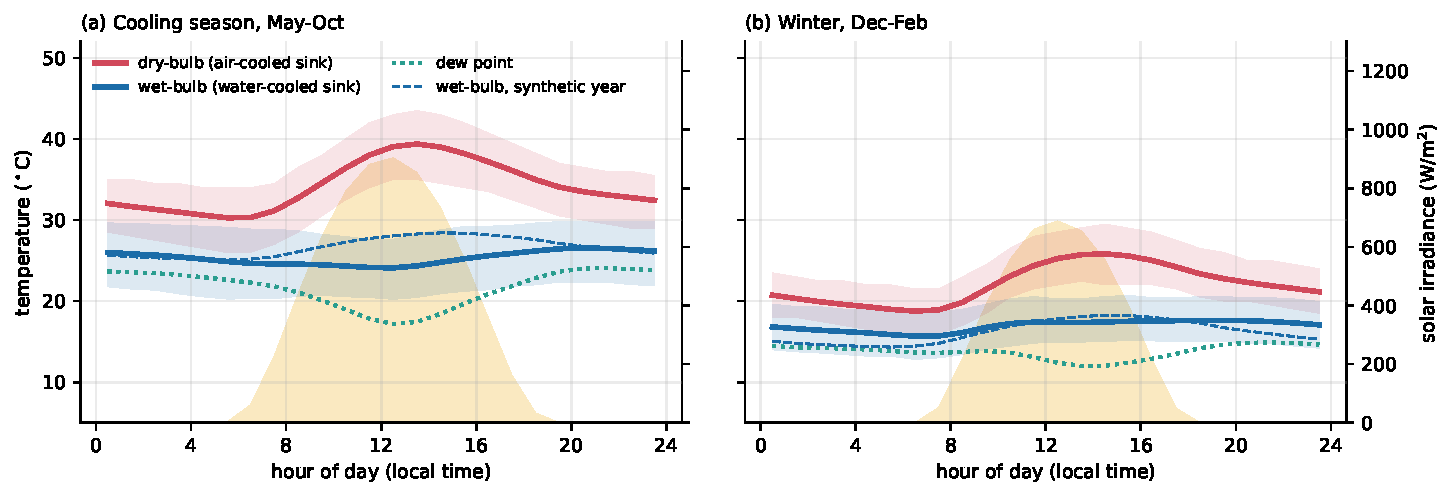
\includegraphics[width=0.92\linewidth]{fig1_heat_sinks.pdf}
\caption{Mean daily cycle of the two heat sinks and of the dew point in the measured Abu Dhabi record (bands: 10--90\%
of days), with irradiance (yellow). Dashed: the wet-bulb of the synthetic year used in the first version of this
report, which rises at midday because its dew point was held constant.}
\label{fig:sinks}
\end{figure}

\section{Results}
\begin{table}[h]\centering\small
\begin{tabular}{@{}lcc@{}}
\toprule
Cooling season (May--Oct), four measured station-years pooled & Air-cooled & Water-cooled\\
\midrule
Heat sink & dry-bulb & wet-bulb\\
Solar-weighted minus night sink temperature, $\Delta T_{\text{sink}}$ (K) & \SwingAC & \SwingWC\\
Night lift $L_{\text{night}}$ (K) & \LiftNightAC & \LiftNightWC\\
\textbf{Carnot penalty $\pi$} (\%) & \textbf{\PiAC} & \textbf{\PiWC}\\
\quad lowest and highest of the four station-years & \PiMinAC{} to \PiMaxAC & \PiMinWC{} to \PiMaxWC\\
Carnot penalty, whole year (\%) & \PiYearAC & \PiYearWC\\
Effective round-trip efficiency of solar-made cold, $\eta_t/(1+\pi)$ (\%) & \EffAC & \EffWC\\
Break-even swing $\Delta T^*$ against an 85\% battery (K) & \SwingStarAC & \SwingStarWC\\
Days on which the tank beats the battery (\%) & \DaysAC & \DaysWC\\
Electricity per MWh of night cooling: grid at night (kWh) & \RouteGridAC & \RouteGridWC\\
\quad solar $\to$ battery $\to$ chiller (kWh) & \RouteBattAC & \RouteBattWC\\
\quad solar $\to$ chiller $\to$ cold tank (kWh) & \RouteTankAC & \RouteTankWC\\
Break-even cleanliness ratio $r^*$ & \RStarAC & \RStarWC\\
Monte Carlo probability that the tank beats the battery & \McWinsAC\% & \McWinsWC\%\\
\bottomrule
\end{tabular}
\caption{Base case. $\pi$ and the efficiency are means of the daily values.}
\label{tab:base}
\end{table}

\begin{figure}[h]\centering
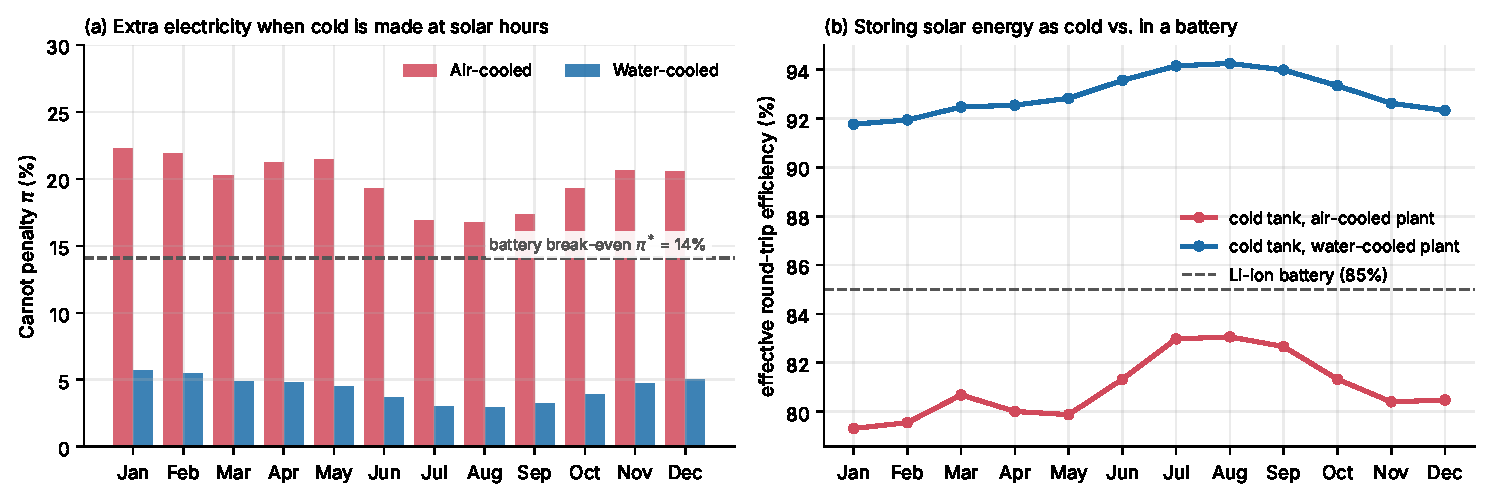
\includegraphics[width=0.97\linewidth]{fig3_penalty_by_month.pdf}
\caption{(a) Carnot penalty by month (bars: mean of the four station-years; whiskers: lowest and highest
station-year). (b) Effective round-trip efficiency of storing solar electricity as cold, against a lithium-ion
battery.}
\label{fig:month}
\end{figure}

\paragraph{Interpretation.}
\emph{Water-cooled plants pay no penalty.} Making cold in the solar hours costs a district-cooling plant
\PiAbsWC\% \emph{less} electricity than making it at night. The penalty is negative from March to November and at most
\PiMonthMaxWC\% in winter (Fig.~\ref{fig:month}). A chilled-water tank then returns \EffWC\% of the solar electricity
put into it: delivering a MWh of night cooling takes \RouteTankWC~kWh of solar electricity through the tank against
\RouteBattWC~kWh through a lithium-ion battery, \SavingWC\% less. The tank itself is plain water: storing 1~MWh of cold
takes $V=Q/(\rho c_p\Delta T)\approx107$~m$^3$ for an 8~K supply--return difference. Since $r^*=$ \RStarWC,
solar-following operation cuts emissions as soon as solar-hour electricity is any cleaner than night electricity.

\emph{Air-cooled chillers tie with the battery.} Their sink is \SwingAC~K hotter in the solar hours, the penalty is
\PiAC\%, and the tank returns \EffAC\%, \BattMinusTankAC{} points below the battery; it wins on \DaysAC\% of
cooling-season days. The measured swing sits just above the break-even swing $\Delta T^*=$ \SwingStarAC~K. On
energy alone the two stores are level within the uncertainty of their own efficiencies (Sec.~\ref{sec:unc}), so for a
building with air-cooled chillers the choice rests on cost and lifetime, which this model does not cover.

\emph{Why the difference?} Both machine types lose 2--3\% of COP per kelvin; what differs is the sink. The dry-bulb
has to rise when the sun shines. The wet-bulb does not, because the same hours bring drier air (Eq.~\ref{eq:twb}).

\emph{Along the coast.} Table~\ref{tab:sets} and Fig.~\ref{fig:sets} apply the same model to every weather data set
we have. The four Abu Dhabi station-years agree closely. In Dubai and Sharjah the midday drop of the dew point is
smaller (\DTdpDubai{} and \DTdpSharjah~K), and the water-cooled penalty is zero in Dubai and \PiWCSharjah\% in
Sharjah: still far below the battery break-even. The air-cooled penalty ranges from \PiACDubai\% in Dubai to \PiACSharjah\% in Sharjah,
on both sides of the break-even, so for air-cooled plant the answer depends on the site.

\emph{Chilled water, not ice.} Lowering the evaporator by 12~K to make ice cuts the effective efficiency to
\IceWC\% (water-cooled) and \IceAC\% (air-cooled). Ice buys a smaller tank at the price of about \IceLossWC{} points of
efficiency.

\begin{table}[h]\centering\small
% Generated by scripts/run_analysis.py -- do not edit by hand.
\begin{tabular}{@{}llccccc@{}}
\toprule
 & & \multicolumn{3}{c}{Solar hours minus night (K)} & \multicolumn{2}{c}{Carnot penalty $\pi$ (\%)}\\
\cmidrule(lr){3-5}\cmidrule(l){6-7}
Weather data, May--Oct & Kind & dry-bulb & dew point & wet-bulb & air-cooled & water-cooled\\
\midrule
Normals-based typical year & synthetic & $+7.3$ & $0.0$ & $+1.7$ & $24.6$ & $+3.5$\\
Reanalysis 2022 & reanalysis & $+7.2$ & $-6.0$ & $-1.5$ & $23.8$ & $-3.0$\\
Reanalysis 2023 & reanalysis & $+7.8$ & $-6.5$ & $-1.8$ & $25.2$ & $-3.5$\\
\addlinespace
Abu Dhabi airport 2022 & measured & $+5.3$ & $-4.5$ & $-1.1$ & $16.9$ & $-2.3$\\
Abu Dhabi airport 2023 & measured & $+5.1$ & $-4.8$ & $-1.5$ & $15.8$ & $-2.9$\\
Abu Dhabi island 2022 & measured & $+4.8$ & $-4.7$ & $-1.5$ & $15.1$ & $-3.0$\\
Abu Dhabi island 2023 & measured & $+4.7$ & $-4.5$ & $-1.5$ & $14.4$ & $-2.9$\\
\addlinespace
Dubai airport 2023 & measured & $+3.6$ & $-1.6$ & $-0.1$ & $10.8$ & $0.0$\\
Sharjah airport 2023 & measured & $+5.5$ & $-2.1$ & $+0.3$ & $17.3$ & $+0.7$\\
\bottomrule
\end{tabular}

\caption{The same calibrated chillers on every weather data set. The synthetic year is the one used in the first
version of this report; the reanalysis is the Open-Meteo product for the Abu Dhabi airport grid cell.}
\label{tab:sets}
\end{table}

\begin{figure}[h]\centering
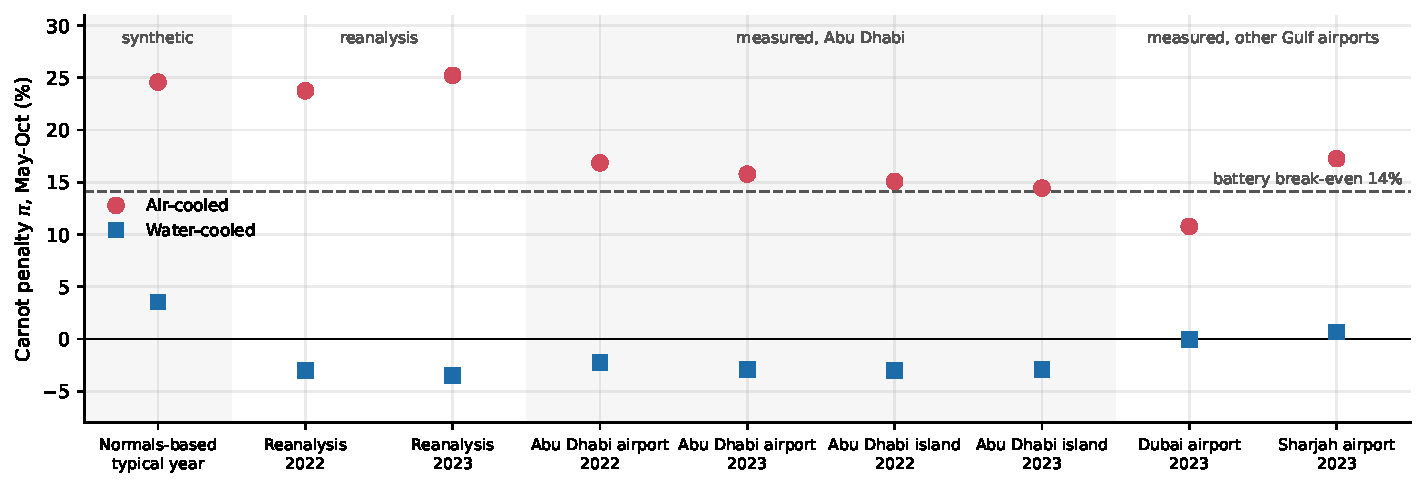
\includegraphics[width=0.9\linewidth]{fig6_all_datasets.pdf}
\caption{Carnot penalty for every weather data set of Table~\ref{tab:sets}. The synthetic year and the reanalysis
overstate the air-cooled penalty, and the synthetic year has the wrong sign for the water-cooled one.}
\label{fig:sets}
\end{figure}

\begin{figure}[h]\centering
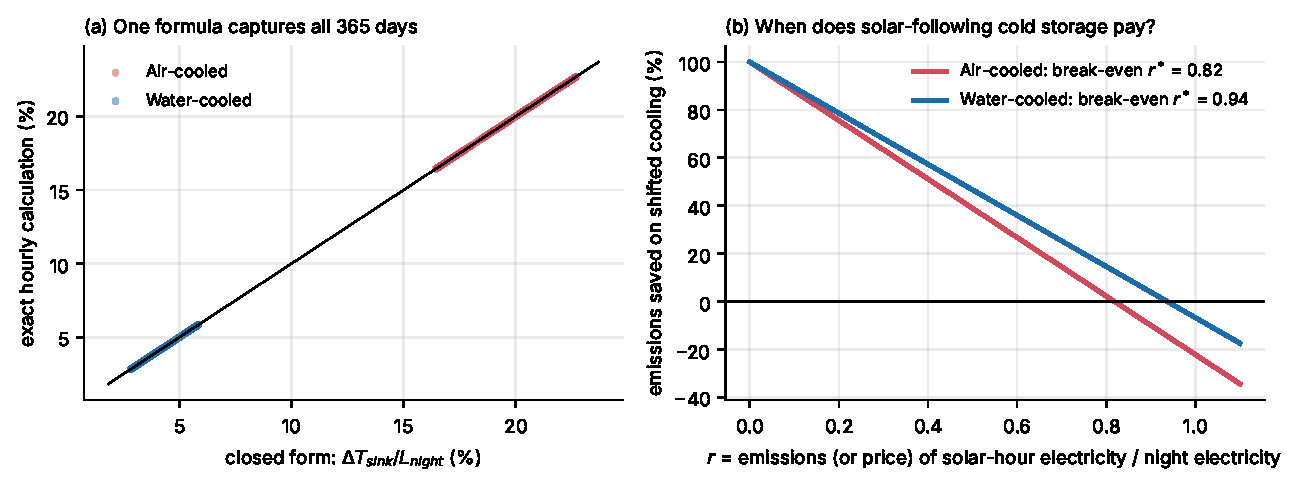
\includegraphics[width=0.86\linewidth]{fig4_closed_form_and_breakeven.pdf}
\caption{(a) The closed form of Eq.~\eqref{eq:pi} against the hour-by-hour calculation for all \NDays{} measured days.
(b) Emissions saved on shifted cooling as a function of how clean solar-hour electricity is relative to night
electricity (Eq.~\ref{eq:clean}).}
\label{fig:cf}
\end{figure}

\section{Uncertainty, sensitivity and verification}\label{sec:unc}
\begin{figure}[h]\centering
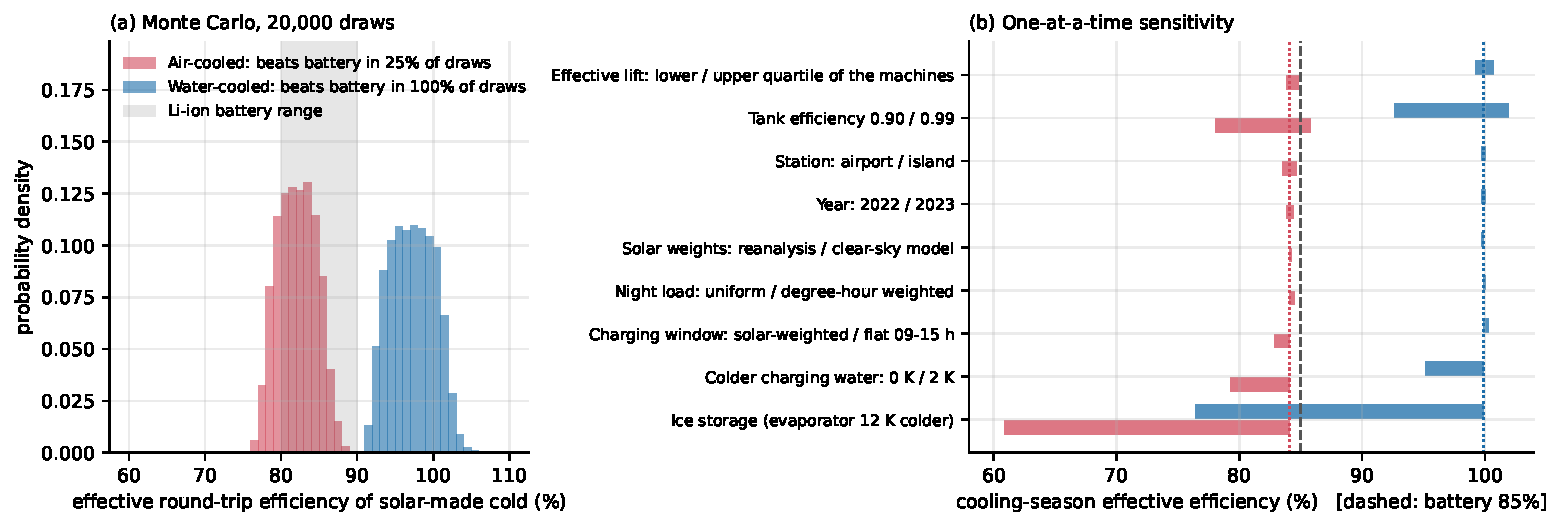
\includegraphics[width=0.97\linewidth]{fig5_uncertainty.pdf}
\caption{(a) Monte Carlo distribution of the effective round-trip efficiency (20\,000 draws). (b) One-at-a-time
sensitivity of the cooling-season efficiency; dotted lines are the base cases (air-cooled red, water-cooled blue).}
\label{fig:unc}
\end{figure}
\paragraph{Monte Carlo.} Each of 20\,000 draws takes: the effective lift of one real machine, picked at random from
the \NWC{} or \NAC{} library machines; $\eta_t\sim U(0.90,0.99)$; $\eta_b\sim U(0.80,0.90)$; and one of the four
measured station-years. For water-cooled plants the tank beats the battery in \McWinsWC\% of draws (efficiency 5--95\%
range \McLoWC--\McHiWC\%, median \McMedWC\%); for air-cooled chillers in \McWinsAC\% of draws
(\McLoAC--\McHiAC\%, median \McMedAC\%). The medians lie below the base case because the sampled tank efficiency
averages 0.945, against 0.97 in the base case.
\paragraph{Sensitivity.} Table~\ref{tab:sens} changes one thing at a time. Apart from making ice, no test brings the
water-cooled tank near the battery's 85\%. The air-cooled tank stays within about two points of the battery under every
change of weather, machine or load shape; what moves it is the tank itself (its efficiency, or colder charging water).

\begin{table}[h]\centering\small
% Generated by scripts/run_analysis.py -- do not edit by hand.
\begin{tabular}{@{}lcc@{}}
\toprule
Effective round-trip efficiency of the cold tank, May--Oct (\%) & Air-cooled & Water-cooled\\
\midrule
Base case & 84.1 & 99.9\\
Effective lift: lower / upper quartile of the machines & 83.8 / 84.8 & 100.7 / 99.2\\
Tank efficiency 0.90 / 0.99 & 78.0 / 85.8 & 92.7 / 101.9\\
Station: airport / island & 83.5 / 84.7 & 99.7 / 100.1\\
Year: 2022 / 2023 & 83.8 / 84.4 & 99.7 / 100.0\\
Solar weights: reanalysis / clear-sky model & 84.1 & 99.7\\
Night load: uniform / degree-hour weighted & 84.5 & 99.9\\
Charging window: solar-weighted / flat 09-15 h & 82.9 & 100.3\\
Colder charging water: 0 K / 2 K & 79.2 & 95.2\\
Ice storage (evaporator 12 K colder) & 60.9 & 76.5\\
\bottomrule
\end{tabular}

\caption{One-at-a-time sensitivity. Two numbers are the two cases named in the row; one number is the changed case.}
\label{tab:sens}
\end{table}

\paragraph{Verification.} Twenty-nine unit tests cover: saturation pressure against steam tables; wet-bulb against
three psychrometric-chart points and against the independent Stull formula~\cite{stull}; bounds (dew point
$\le T_{wb}\le T$); the two-term response of Eq.~\eqref{eq:twb} against the full balance and against its analytic
coefficients; $s=1/L_0$; the closed form against brute force; the break-even algebra; the library reader on a
hand-made file with a known answer and on both real libraries; and the six station-years (complete, physically
bounded, in local time). The analysis itself stops if a fitted chiller would exceed the Carnot COP in any measured
hour.

\section{What testing against measurements changed}\label{sec:changed}
The version of this report submitted on 13 November used a synthetic typical year, built from monthly climate normals
with the dew point held constant through the day, and design values for the air-cooled chiller. It gave
$\pi=$ \FirstPiAC\% for air-cooled and \FirstPiWC\% for water-cooled plants. Three things changed when the model met
measurements.
\begin{itemize}
\item \textbf{The humidity cycle.} The measured dew point falls by \DTdpAbs~K in the solar hours; the synthetic year
had no such cycle. This is what turns the water-cooled penalty from \FirstPiWC\% into a bonus.
\item \textbf{The nights.} The daily maxima of the normals table we had used are on average \NormTmaxDiff~K below
the 2022--2023 airport record, but its daily minima are \NormTminDiff~K below it (\NormTminDiffLo--\NormTminDiffHi~K
by month). The synthetic year therefore had too large a day--night swing: \FirstDTdb~K instead of \DTdb~K. With the
measured weather alone, the air-cooled penalty would fall from \FirstPiAC\% to \FirstPiACMeasuredWeather\%.
\item \textbf{The air-cooled machines.} Real ones lose \SensAC\,\%/K, about \DesignUnderAC\% more than the 2.2\,\%/K
of our design values. With that alone, the penalty would rise from \FirstPiAC\% to \FirstPiACLibraryChiller\%.
\end{itemize}
The two air-cooled corrections pull in opposite directions and leave \PiAC\%. A reanalysis, which we tried first as a
check, reproduces the humidity cycle but shares the too-cool nights (Table~\ref{tab:sets}): it would have confirmed
the wrong air-cooled number. Only station observations settled it.

\section{Limitations and next steps}\label{sec:lim}
\begin{itemize}
\item \textbf{Two years, two stations.} The four station-years agree closely, but Dubai and Sharjah show that the
humidity cycle is local. A plant should be assessed with the record of its own site, and a longer record would show
how much the result varies from year to year.
\item \textbf{Full-load curves.} We ignore part-load operation and the loss of chiller capacity on hot afternoons.
Gulf wet-bulbs of 30$\C$ are at the edge of the library curves' range.
\item \textbf{Fixed tower approach.} A real cooling tower's approach widens as the wet-bulb falls, so the condenser
water follows the wet-bulb less than one for one. That would shrink the water-cooled bonus somewhat; it does not
change its sign.
\item \textbf{The tank.} $\eta_t=0.97$ assumes a well-stratified tank; with $\eta_t=0.90$ the water-cooled tank still
beats the battery but the air-cooled one clearly does not (Table~\ref{tab:sens}).
\item \textbf{Energy only.} We ignore tank and battery cost, the water a cooling tower evaporates, and pump and fan
power.
\item \textbf{Scale.} Translating the result into GWh for Abu Dhabi needs hourly cooling-load and dispatch data that
are not public; Eq.~\eqref{eq:clean} is written so that a utility can plug in its own numbers.
\end{itemize}

\section{Conclusion}
The thermodynamic price of following the sun with cooling is one number, $\pi=\Delta T_{\text{sink}}/L_{\text{night}}$.
Measured in Abu Dhabi it is about \PiWC\% for water-cooled district-cooling plants, whose heat sink is the wet-bulb
temperature and is coolest when the sun is up, and about \PiAC\% for air-cooled chillers, level with the losses of a
battery. The practical message for the UAE is that chilled-water tanks at district-cooling plants are a better home
for surplus solar electricity than batteries; that for air-cooled buildings the two stores tie on energy, so cost must
decide; and that making ice gives away about \IceLossWC{} points of efficiency.

\section*{Reproducibility}
Everything is in the submission folder: \texttt{src/carnot\_penalty.py} (model), \texttt{scripts/} (weather builders
and analysis), \texttt{tests/} (29 tests), \texttt{data/} (inputs with provenance) and \texttt{results/} (outputs).
\texttt{bash reproduce.sh} regenerates every number, table and figure in under a minute; the run is deterministic
(seed 2026) and needs no network access. The numbers in this text are not typed: the analysis writes them into
\texttt{report/numbers.tex}, which this document reads.

\section*{Use of tools and AI}
Python (NumPy, pandas, Matplotlib, pytest) and \LaTeX. As the competition rules ask, we disclose that an AI assistant
(Anthropic's Claude) was used in this work: for framing the problem and developing the model, for writing the code and
its tests, for finding and preparing the input data and the figures, for testing the first version against measured
weather and a second chiller library (the corrections in Section~\ref{sec:changed}), and for drafting and typesetting
the report.
The work is set up so that its results do not have to be taken on trust. Every result and figure is regenerated by
the open code in the submission folder; the model is checked by 29 unit tests against independent references; the
closed form is checked against the hour-by-hour calculation; and the weather and both chiller libraries are public
data with their sources given in \texttt{data/README.md}. The team is responsible for the content and for defending
it.

\begin{thebibliography}{99}\small
\bibitem{iea} International Energy Agency (2018). \emph{The Future of Cooling}. IEA, Paris.
\bibitem{rtc} Masdar and EWEC (January 2025). Announcement of a 5.2~GW solar PV and 19~GWh battery project in Abu Dhabi to deliver 1~GW of round-the-clock power.
\bibitem{wang2020} Wang, Y., Hua, Q., Sun, L. and Liu, Q. (2020). Thermodynamic efficiency comparison between thermal and electric storage for photovoltaic-driven chilling system. \emph{J. Energy Storage} 28, 101253.
\bibitem{wangdennis} Wang, X. and Dennis, M. (2018). A comparison of battery and phase change coolth storage in a PV cooling system under different climates. \emph{Sustain. Cities Soc.} 36, 92--98.
\bibitem{luerssen} Luerssen, C., Gandhi, O., Reindl, T., Sekhar, C. and Cheong, D. (2020). Life cycle cost analysis (LCCA) of PV-powered cooling systems with thermal energy and battery storage for off-grid applications. \emph{Appl. Energy} 273, 115145.
\bibitem{alaali} Al-Aali, I. and Modi, V. (2022). Decarbonizing the electricity sector in Qatar using PV combined with ice thermal and battery storage. \emph{Energy Strategy Rev.} 44, 101014.
\bibitem{ashrae} ASHRAE (2021). \emph{ASHRAE Handbook---Fundamentals}, Ch.~1 (Psychrometrics).
\bibitem{magnus} Alduchov, O.~A. and Eskridge, R.~E. (1996). Improved Magnus form approximation of saturation vapor pressure. \emph{J. Appl. Meteorol.} 35, 601--609.
\bibitem{atb} National Renewable Energy Laboratory (2024). \emph{Annual Technology Baseline}: utility-scale battery storage (85\% round-trip efficiency).
\bibitem{openmeteo} Zippenfenig, P. (2023). \emph{Open-Meteo.com Weather API}. Zenodo, doi:10.5281/zenodo.7970649. Historical Weather API, \url{https://open-meteo.com}, accessed 13 November 2026.
\bibitem{haurwitz} Haurwitz, B. (1945). Insolation in relation to cloudiness and cloud density. \emph{J. Meteorol.} 2, 154--166.
\bibitem{eplus} U.S. Department of Energy. \emph{EnergyPlus}, datasets \texttt{Chillers.idf} and \texttt{AirCooledChiller.idf}, and Engineering Reference. \url{https://github.com/NREL/EnergyPlus}
\bibitem{hydeman} Hydeman, M. and Gillespie, K.~L. (2002). Tools and techniques to calibrate electric chiller component models. \emph{ASHRAE Transactions} 108(1).
\bibitem{gordon} Gordon, J.~M. and Ng, K.~C. (2000). \emph{Cool Thermodynamics}. Cambridge International Science Publishing.
\bibitem{iem} Iowa Environmental Mesonet, Iowa State University. ASOS/METAR archive of airport weather observations, stations OMAA, OMAD, OMDB and OMSJ. \url{https://mesonet.agron.iastate.edu/request/download.phtml}, accessed 13 November 2026.
\bibitem{stull} Stull, R. (2011). Wet-bulb temperature from relative humidity and air temperature. \emph{J. Appl. Meteorol. Climatol.} 50, 2267--2269.
\end{thebibliography}
\end{document}
